\maketitle

나의 삶은 20세기 말 대한민국 서울에서 태어나 경기도에서 자란 20대 남성의 삶이기도 하다. 키, 몸무게, 소득, 자산, 수능 점수, 학점 등 정량적인 지표를 이용해 저 멀리서 평균을 낸 20대 남성의 삶에 내가 얼마나 가까운지 알아볼 수도 있을 것이다. 하지만 그보다는 생애과정에서 내가 세상과 어떻게 상호작용을 했는지, 어떤 사건에서 사회적 기준을 충족하거나 충족하지 못했는지 살펴보는 것이 나에게는 더 의미가 있을 것 같다.

이 글에서는 나의 지난 삶을 영유아기, 아동기, 청소년기, 성인기로 나눠 생애과정의 단계별로 돌아보려 한다. 그리고 각 단계에서 나를 둘러싼 환경과 어떻게 상호작용했는지, 그런 상호작용이 개인적으로, 또 사회적으로 어떤 의미를 가졌는지 짚어보고자 한다.

\section*{영유아기: 가족과의 유대감}

UN에 따르면 1998년 한국의 영아 사망률은 7.4\%였다\footnote{United Nations, ``World Population Prospects 2022'', <United Nations>, 2022, <https://population.un.org/wpp/>, (접근일자: 2022.12.10).}. 부모님은 내가 태어나기도 전에 내 이름을 지었고, 어머니는 모차르트 음악을 들으며 태교했다. 부모님이 맞벌이를 했기에 어렸을 적의 나는 할머니, 할아버지와 보내는 시간이 더 많았다. 조금 이르게 들어간 유치원에는 잘 적응하지 못했다. 한 번은 내가 유치원에서 무언가를 쏟았는데, 보육교사가 나를 심하게 혼낸 일이 있었다. 부모님은 이를 계기로 `믿을만한 보육 시설'을 찾은 끝에 나를 집에서 조금 떨어진 공동육아 어린이집에 보냈다.

부모님이 공동육아 어린이집을 선택한 또 다른 이유는 늦은 시각까지도 아이들을 맡아줬기 때문이었다. 해가 지고 친구들이 하나둘 집으로 돌아갈 때도 나는 혼자 남곤 했다. 한국 사회에서는 영유아와 부모 사이의 유대감을 중요하게 여긴다. 이 시기에 욕구를 제대로 충족하지 못하면 성인이 된 후에도 영향을 미친다고 한다. 성인들은 현재 겪는 심리적 문제를 자신의 영유아기에서 찾아본다. 생애과정에서 영유아기의 중요성이 강조되다 보니 최근에는 영유아에게 외국어 능력을 요구하기까지도 한다.

\begin{figure}[h]
  \centering
  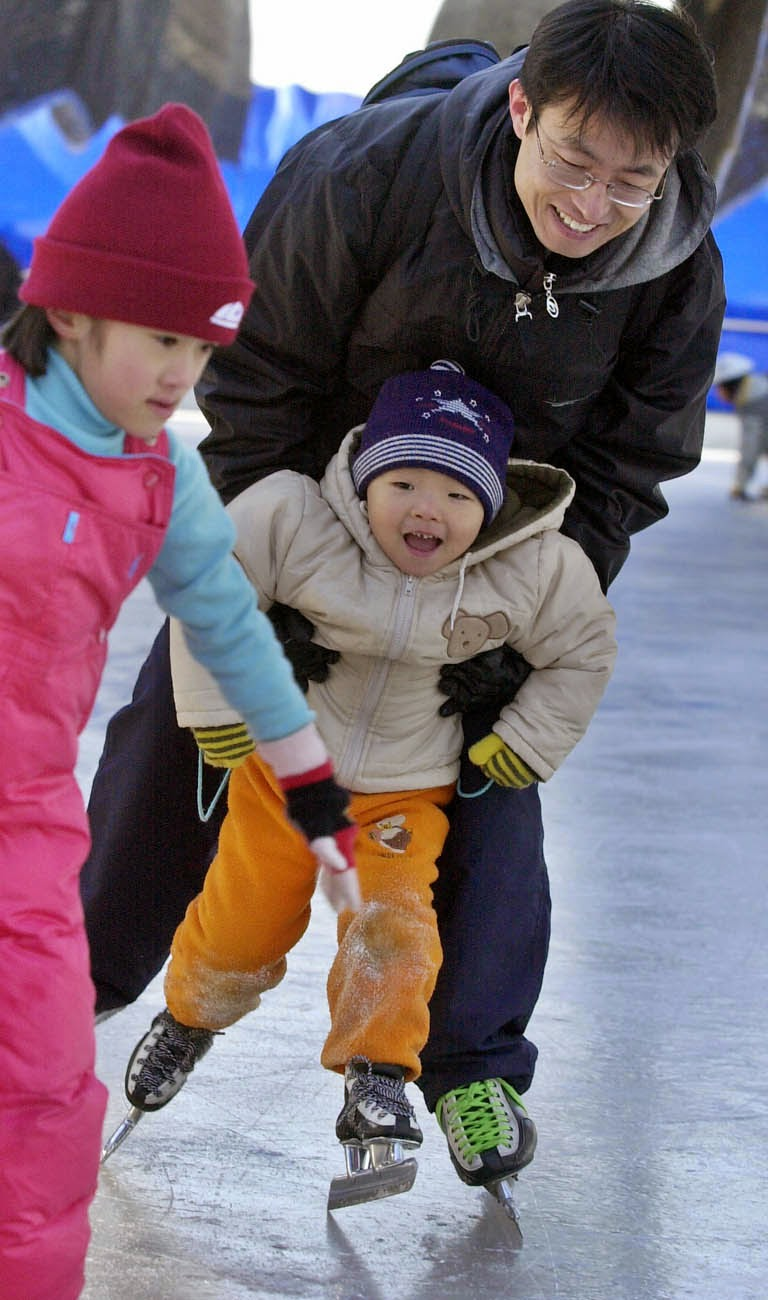
\includegraphics[width=7cm]{donga2001.jpg}
  \caption[]{아버지와 스케이트를 타는 영유아기의 나. 2001년 12월 30일 촬영\footnotemark.}
\end{figure}

\footnotetext{``[사회 포토] ``아빠, 하나도 안추워요'''', <동아일보>, 2001, <https://www.donga.com/news/article/all/20011230/7774271/1>, (접근일자: 2022.12.10).}

나는 부모님을 아침과 저녁에만 만날 수 있었지만, 유대감에 큰 문제는 없었다. 주말에는 여기저기로 외출을 했다. 아버지는 특히 신경 써서 나와 시간을 보냈다. 안정적인 직장이 있던 부모님은 외환위기의 타격을 피할 수 있었고, 나는 안전한 환경에서 자란 편이었다. 다만 혼자 있는 걸 선호하는 지금의 독립적인 성격이 이 시기와 무관하지 않을지도 모른다는 생각이 든다.

\section*{아동기: 규칙과 또래 집단}

``애들은 패야 말을 듣는다''라는 표현에 동의하는 사람이 대다수였는지, 2000년대 중반까지도 많은 학교에서 일상적으로 체벌을 했다. 강압적인 교육 환경이 싫으셨던 부모님은 나를 집에서 한참 떨어진 사립 초등학교에 보내기로 했다. 치열한 경쟁을 뚫고 입학한 학교는 정해진 규칙을 성실히 따를 것을 요구했다. 그 과정에서 각종 이데올로기를 접했다. 매주 월요일에는 전교생이 강당에 모여 애국가를 부르고 ``조국과 민족의 무궁한 영광을 위하여 몸과 마음을 바쳐 충성을 다할 것을 굳게 다짐''하는 맹세를 했다. 수업에서는 언제 어떻게 행동해야 하는지, 무엇이 옳고 그른지, 어떤 어린이가 착한 어린이인지 배웠다. 학교의 규칙은 압박이 되기도 했다. 심리적인 이유로 등굣길에 구토감을 느끼는 일이 잦았다. 그래도 나는 나름대로 착한 어린이가 되기 위해 노력했다. 어른들이 하라는 것은 안 해도, 적어도 하지 말라는 것을 하지는 않았다. 가족은 칭찬으로, 학교는 성적표로 노력을 보상했다.

학교에서는 또래 집단이 너무나 중요했다. 또래 집단에 소속되기 위해서는 외모, 태도, 말투, 행동 등의 기준에서 내가 그들과 다르지 않다는 것을 보여야 했다. 위화감이 들면 비난을 받고 무리에서 배제될 수 있었다. 또래 집단이 제시하는 여러 기준 중 하나는 성별이었다. 어린이집과 달리 초등학교에서는 남자아이들과 여자아이들이 따로 놀았고, 각자의 문화가 철저히 분리되어 있었다. 만약 남자아이가 여자아이들과 놀거나, 여자아이들이 하는 놀이를 하면 남성 또래 집단으로부터 조롱을 받았다. 나는 동성 또래 집단의 보이지 않는 기준을 충족하기 위해 나 스스로를 점검해야 했다. 이후에는 점검을 넘어, 능동적으로 남자다운 것과 여자다운 것, 남자가 할 일과 여자가 할 일이 다르게 정해져 있다는 구분을 지었다. 덕분에 나는 안정적으로 무리에 속할 수 있었다. 또래 집단은 나로 하여금 스스로를 정체화하고, 인식하게 만들었다. 그 대가는 성 역할 고정관념이었다. 이것이 고정관념임을 의식한 계기는 훗날의 교육이었다.

\section*{청소년기: 진로와 대학 진학}

초등학교를 졸업한 뒤, 공교육이 대학 입시에 매몰되어 있다고 생각하신 부모님은 나를 대안학교에 보냈다. 서류전형에 캠프전형, 면접전형까지 거치며 합격한 중학교였다. 학교에 다니기 위해 경기도로 이사를 했다. 학교의 교육 과정은 대학 진학보다는 다양한 진로와 가능성을 탐색하는 데 초점이 맞춰져 있었다. 다른 중학교의 학생들과 달리 사교육을 받지도, 이른 대학 입시의 압박을 받지도 않았다. 다만 학교는 3년 안에 내가 진로의 방향을 결정하길 기대했다. 그 기대에 부응하고자 한 것은 아니지만, 자유로운 환경에서 나는 컴퓨터 프로그래밍을 접했다. 프로그래밍은 놀이이자 취미, 특기였다. 중학교 3학년 때 직접 만든 웹 서비스는 학교 안팎으로 화제가 되기도 했다. 가족과 학교가 나에게 기대한 진로 탐색을 성공적으로 이룬 셈이었다. 또래에게는 ``하고 싶은 걸 일찍 찾아낸 네가 부럽다''라는 말을 자주 듣곤 했다.

\begin{figure}[h]
  \centering
  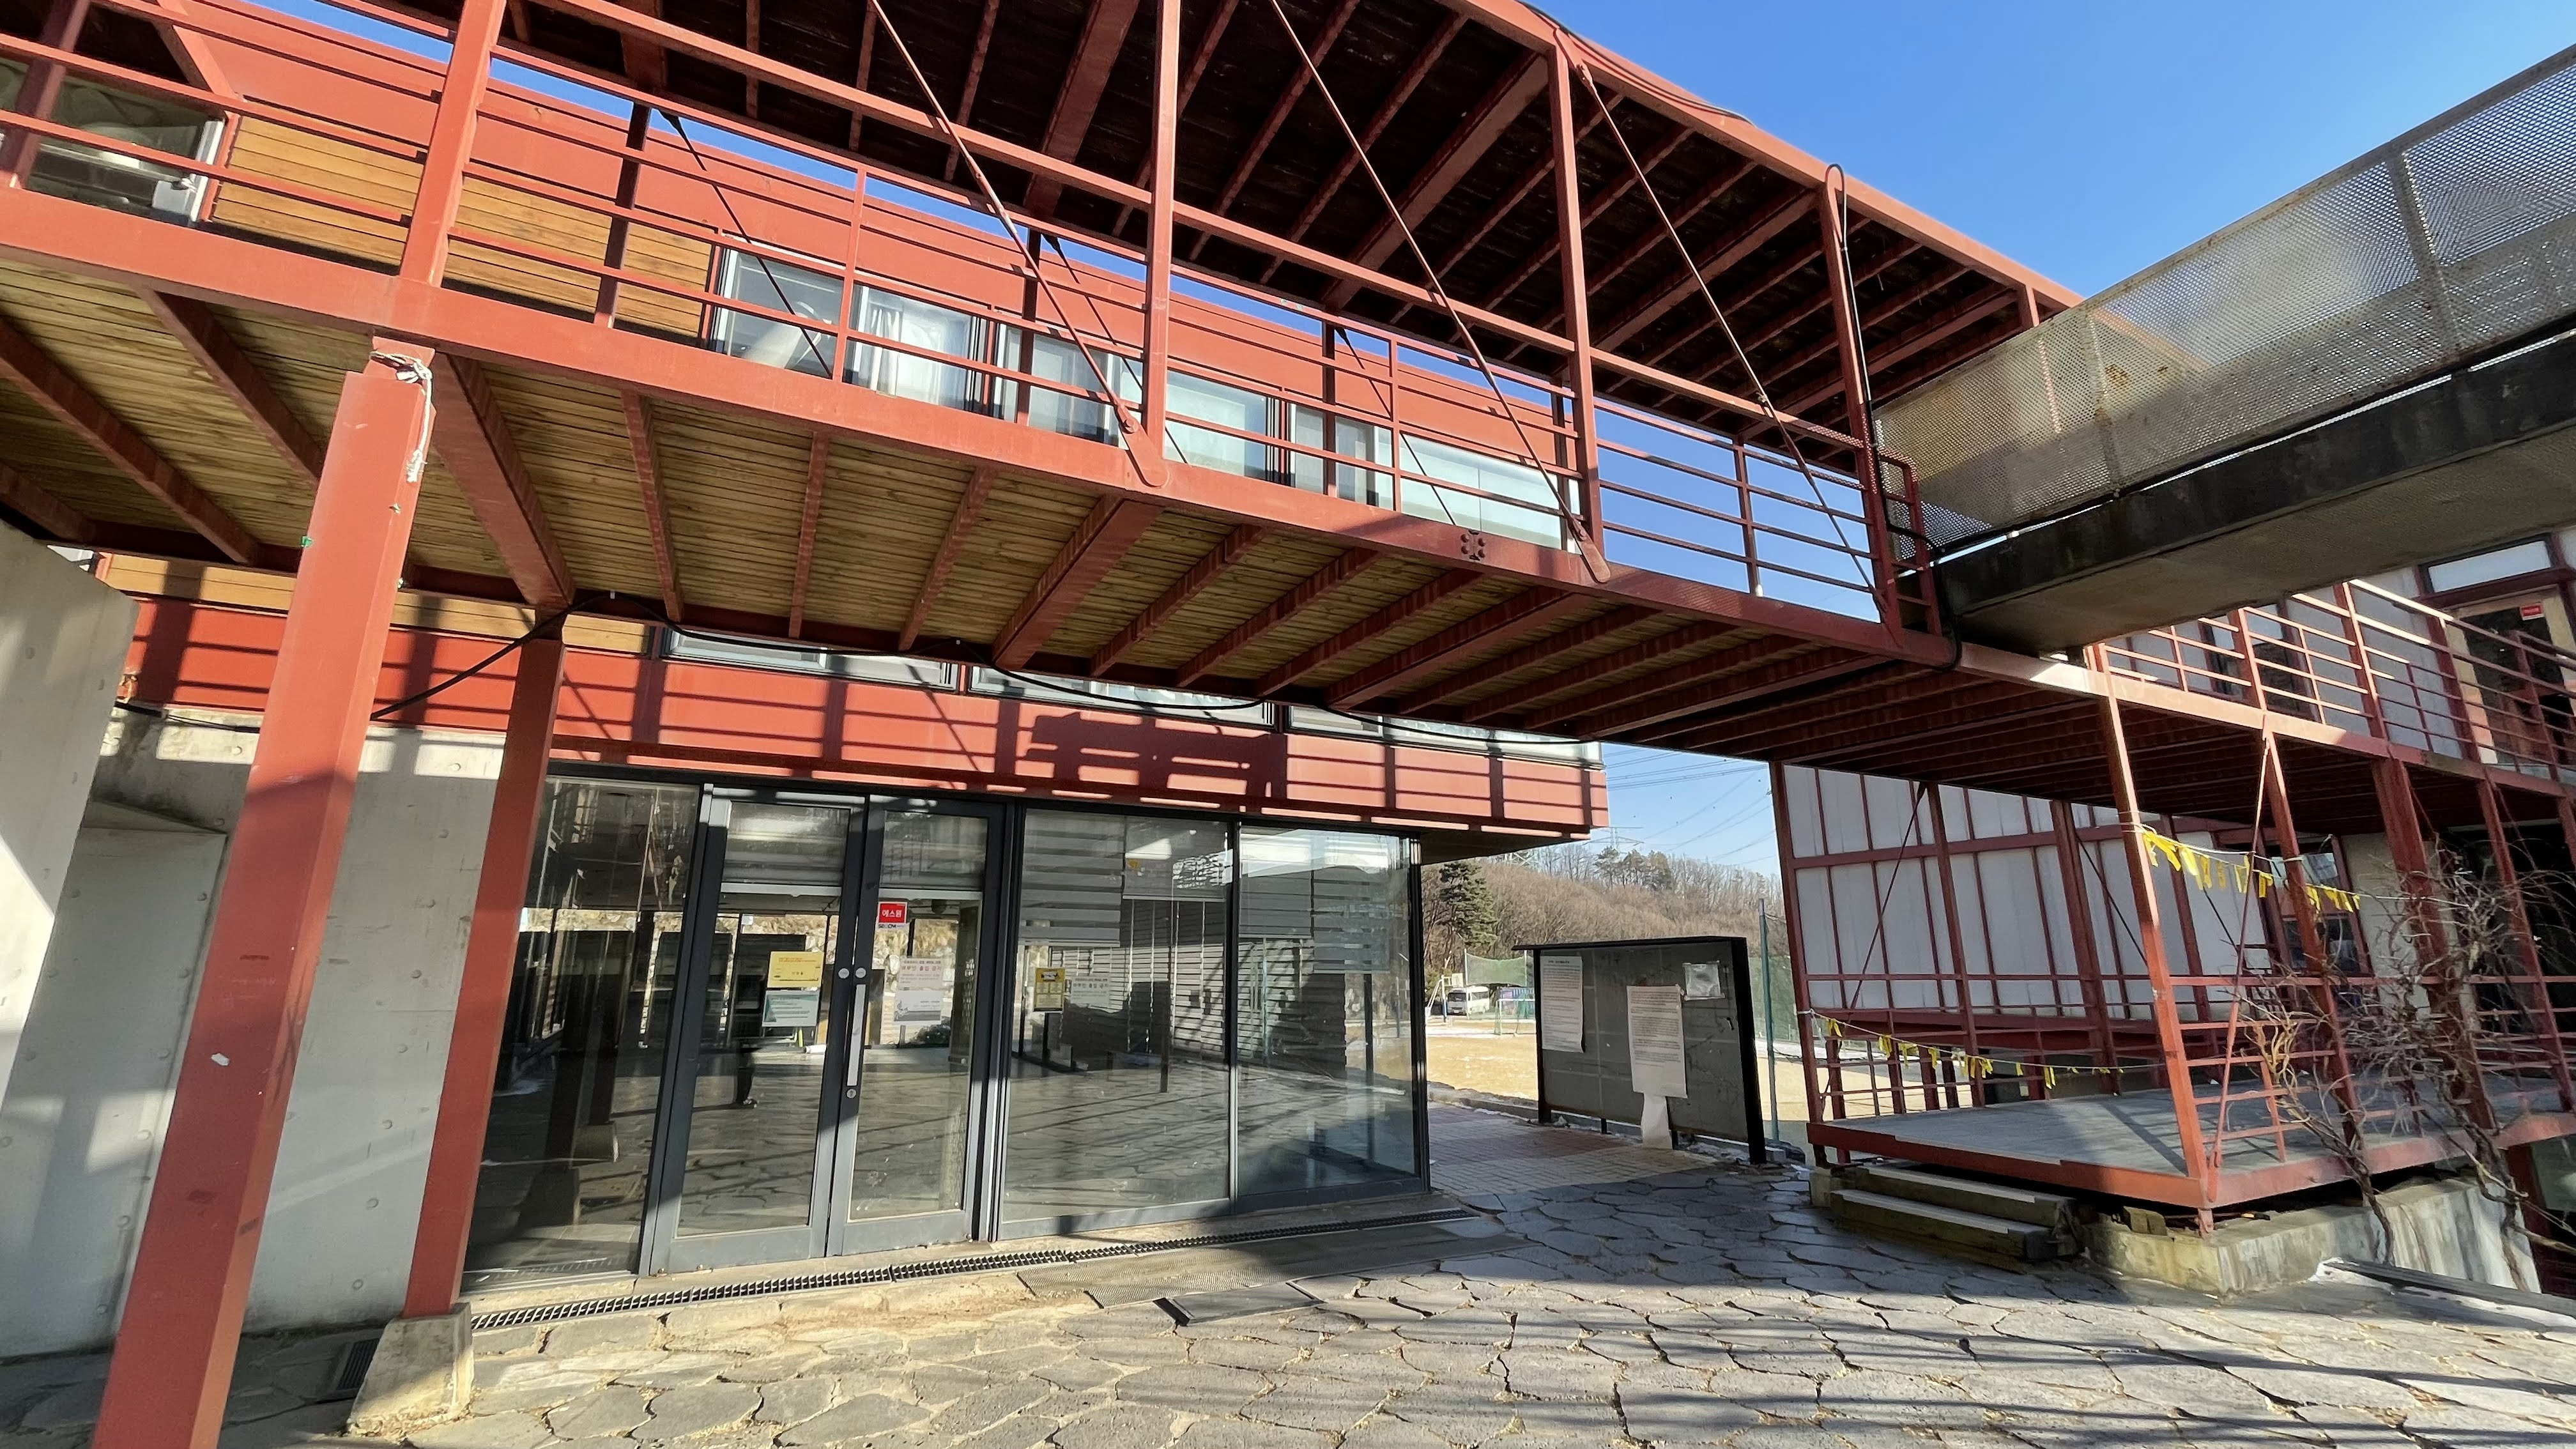
\includegraphics[width=7.4cm]{ewoo2022-1.jpg}
  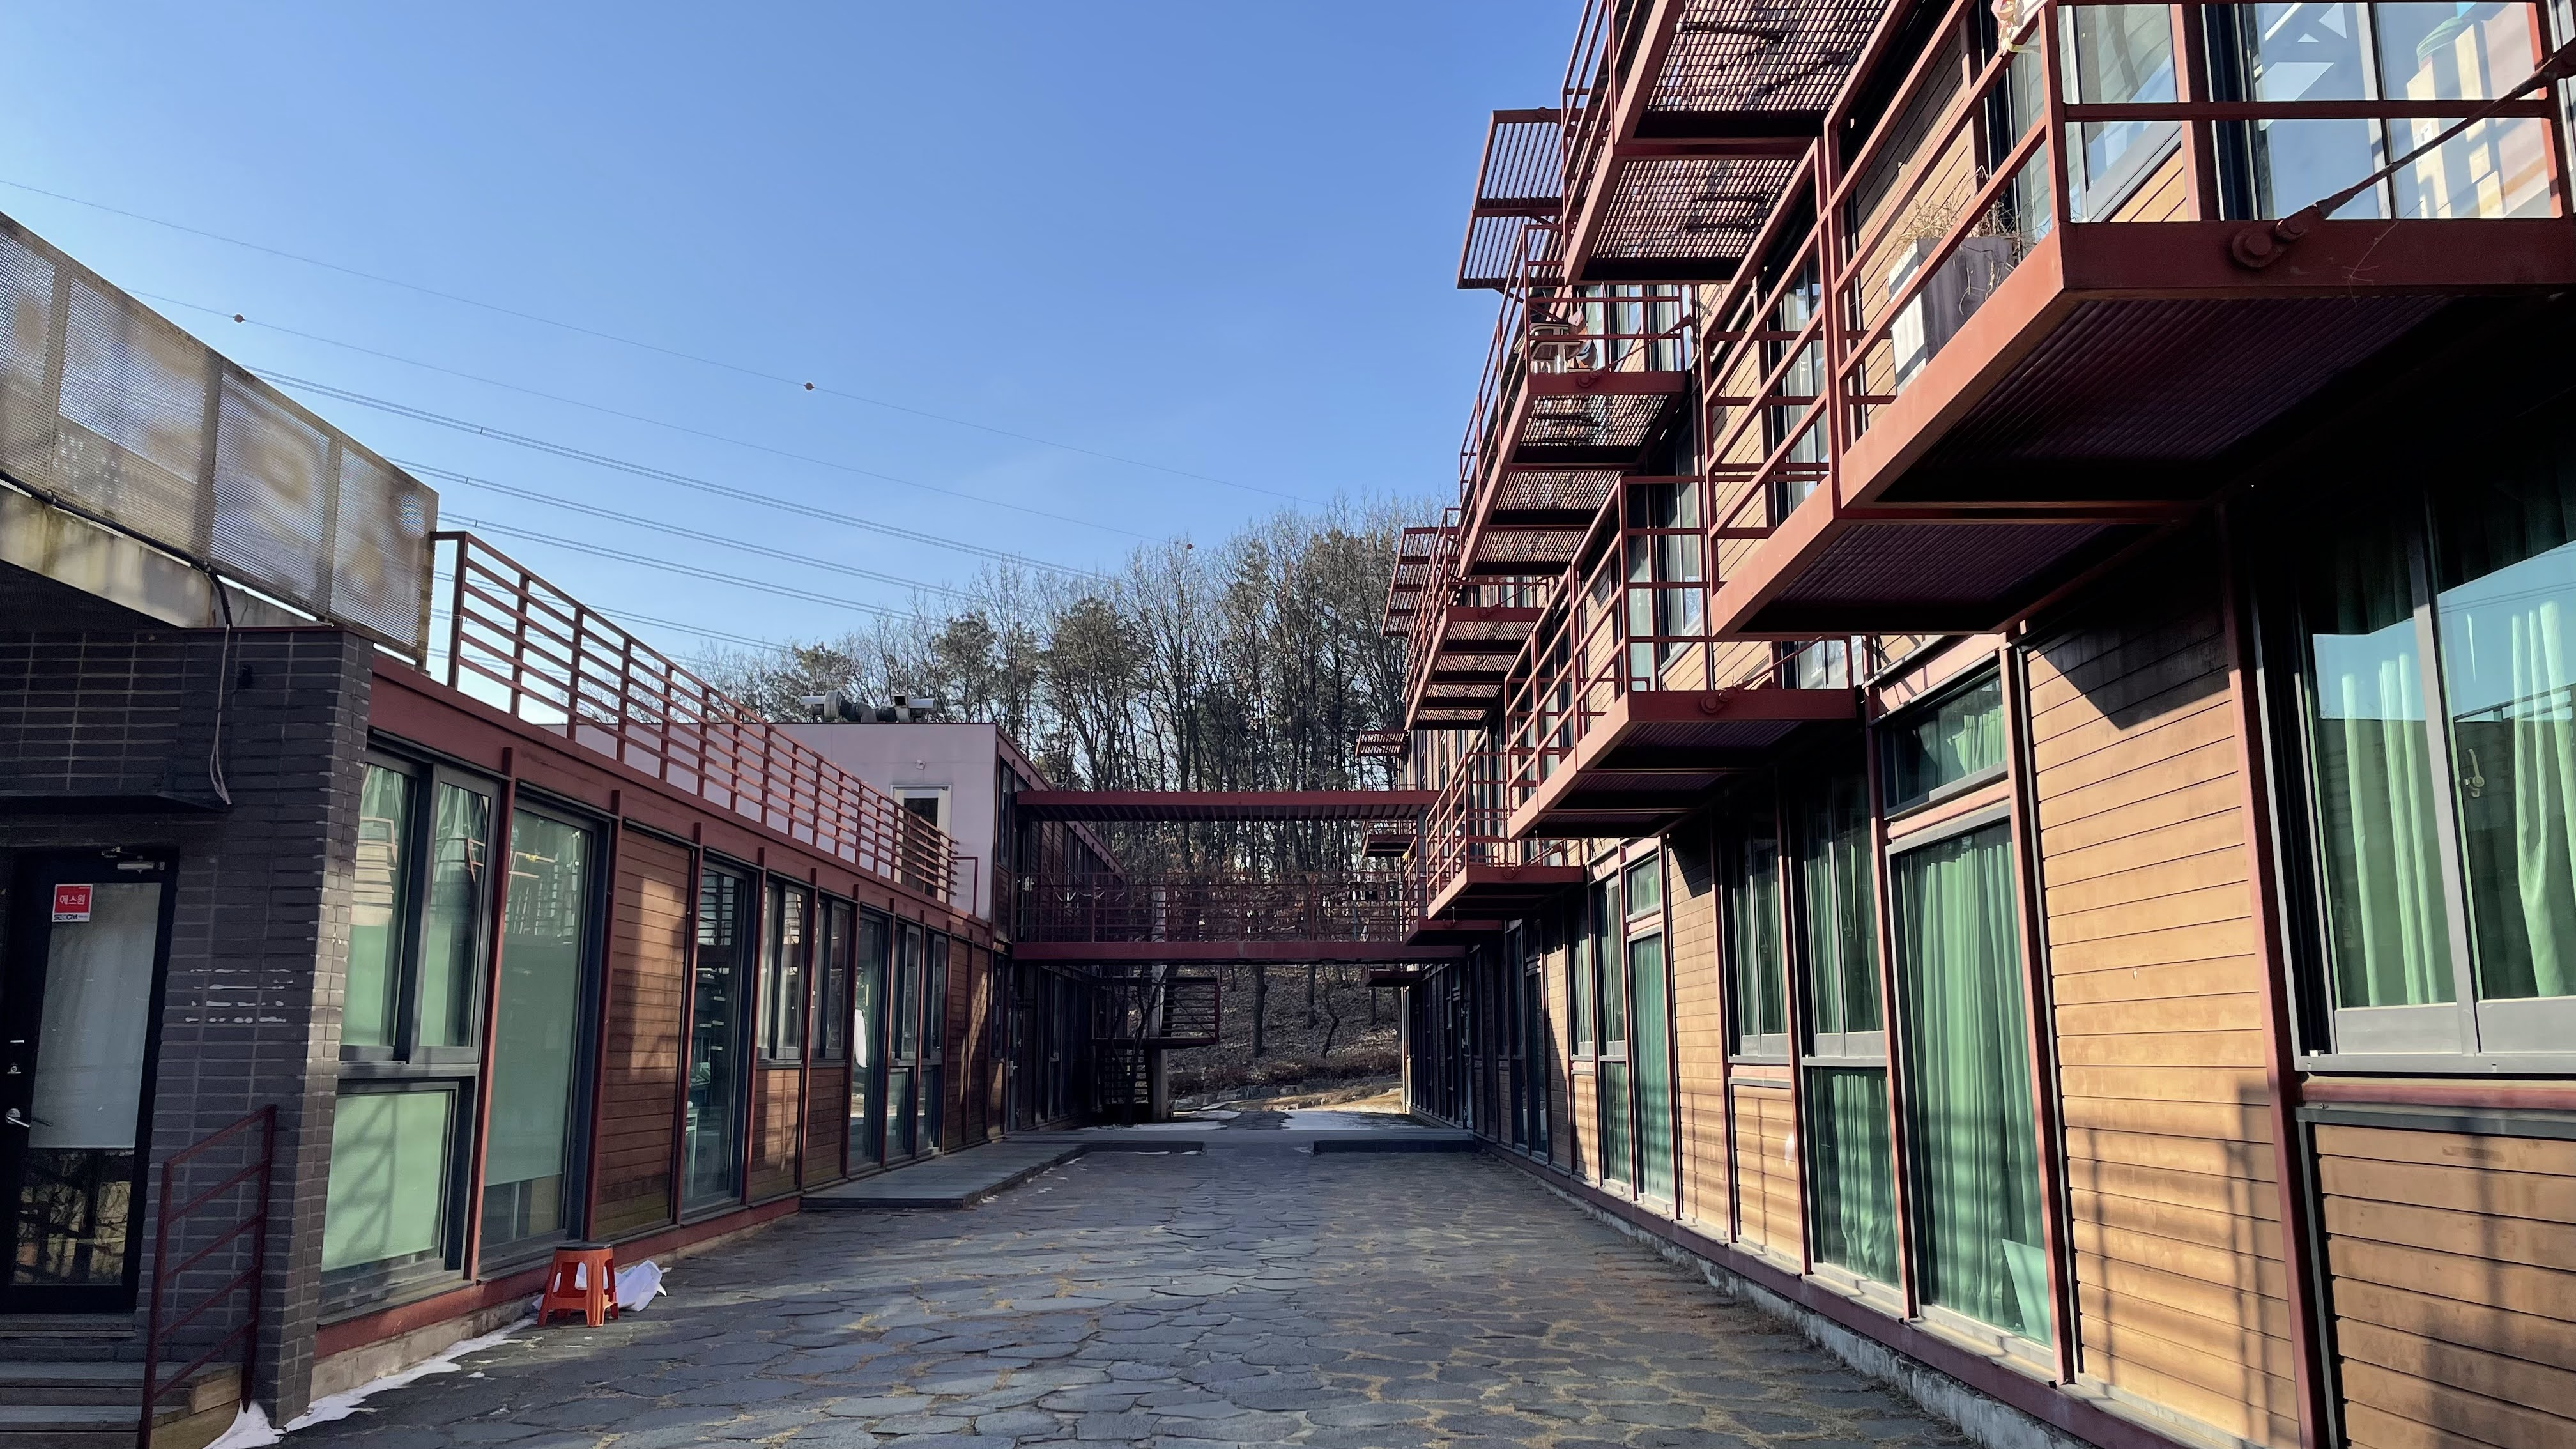
\includegraphics[width=7.4cm]{ewoo2022-2.jpg}
  \caption{내가 청소년기를 보낸 중고등학교의 모습. 2022년 1월 12일 촬영.}
\end{figure}

고등학교 역시 같은 계열의 대안학교로 진학했다. 학교의 교육 과정은 사회의 지배 이데올로기를 비판적으로 분석하는 방향으로 구성되어 있었다. 교내 어디에서도 태극기를 찾아볼 수 없다는 사실을 이때야 깨달았다. 학교는 대학 입시 위주의 교육을 비판하면서 대학 진학이 아닌 또 다른 길이 있음을 교육했다. 그런데 고등학교 3학년이 되자 학교가 돌변했다. 대안 교육의 성공을 입증하는 데 명문대 진학률이 강력한 증거가 될 것이라는 추론은 어렵지 않았다. 주변의 기대도 완전히 달라져 있었다. 가족, 친척, 심지어 친구들까지 내가 서울에 소재한 4년제 종합대학에 진학하길 기대했다. 내 주변뿐만이 아니었다. 전 사회가 나서서 대학에 진학할 것을 요구했다. 한국에서 대학 진학은 성인으로 가는 입사의례다. 그 의례를 본격적으로 준비하는 1년의 시기는 `고3'이라는 특수한 신분으로 격리된다. 성인기(때로는 그 이후까지)의 신분을 결정하는 의례이기 때문에 수능 듣기 평가 중에는 공항에 항공기도 이착륙하지 않는다. 대학에 대한 온갖 신화와 고졸에 대한 온갖 괴담 속에서 고통스러운 1년을 견디는 것이 한국에서는 너무나 중요하다.

대학에 대해 생각해본 적이 없던 나에게는 낯선 환경 변화였다. 하지만 주변의 기대에 부응하고, 사회에서 어엿한 성인으로 인정받기 위해서는 고행의 시간을 보내야 했다. 스무살이 된 해, 대학에 합격한 아이들은 축하와 격려를 받으며 당당하게 성인이 되었다. 어느 대학에도 합격하지 못한 아이들은 성인의 권리를 충분히 누리지도 못한 채 내년에 다시 치러질 입사의례를 준비했다. 한편 대학에 진학하지 않기로 결정한 아이들은 그대로 사회에 내던져졌다. 인문계 고등학생의 대학 진학을 전제한 사회에는 그들을 위한 자리가 없었다. 고등학교 졸업 후 대학에 진학하지 않은 한 친구는 끊임없이 ``그래도 대학은 가야 하지 않겠냐"는 주변의 압박을 받는다고 말했다. 그런 압박을 견디지 못한 아이들은 남들에 비해 뒤처졌다는 불안감을 안고 다시 대학 진학을 준비하곤 했다.

\section*{성인기: 가치관의 타협과 취업}

미디어는 스무 살을 찬란하게 묘사한다. 스무 살은 두 번 다시 오지 않을 가장 반짝이는 나이이며, 모든 가능성이 열려있는 나이이고, 하루하루가 가슴뛰어야 하는 나이다. 하지만 현실에 미디어가 그려내는 스무 살은 없었다. 스무 살의 나는 서울이 아닌 경기도에 소재한 4년제 대학교에 입학하여 축하와 동경, 무시와 멸시를 동시에 받았다. 촘촘하게 서열화된 대학의 피라미드에서 나는 지난 입사의례로 정해진 나의 자리를 더듬거리며 찾아가고 있었다.

스무 살의 내가 대학 사회의 진정한 일원으로 인정받으려면 합격증만으로는 부족했다. 입학 전 `예비 신입생 환영회'부터 입학 후 `신입생 환영회', `새내기 배움터' 등 온갖 행사에 빠짐없이 참석하며, 가고 싶지도 않은 술자리를 굳이 찾아가며, 각종 동아리에 가입해 활동하며, 내가 대학 사회와 어울리는 인간임을 증명하기 위해 부단히 애썼다. 하지만 대안학교에서 청소년기 전체를 보낸 나의 가치관과 내가 마주한 새로운 사회의 가치관은 너무나도 달랐다. 나는 대안학교의 흔적을 씻어내고 나의 모난 부분을 둥글게 깎아내야만 했다. 대학 사회의 낯선 규칙을 내면화하고 가치관을 타협하는 사회화에는 1년 넘는 시간이 필요했다.

이제는 사회가 20대에게 부과한 과업을 무시할 수 없었다. 한국 사회는 아무리 늦어도 서른 살 전에는 첫 직장에 취업할 것을 요구한다. 군 복무를 마친 남성은 적어도 28살에는 취업해야 늦었다는 말을 듣지 않는다. 여성은 26살에 취업해도 늦었다는 핀잔을 듣는다. 이제 막 청소년기의 과업을 마친 새내기들에게 학교는 취업을 강조했다. 전공필수 과목에서는 미래의 이력서를 작성하는 과제를 했다. 대기업에 취업한 선배들이 발표하는 특강을 듣기 위해 주말에도 학교에 가야 했다. 교수님들은 수업 중 `성공한' 선배들의 사례를 자랑스럽게 나열하곤 했다. 여기서 `성공'이란 당연히 대기업에 입사해서 높은 연봉을 받는 것을 의미했다. 속수무책으로 저학년과 고학년의 경계에 서게 되자 취업 압박은 더욱 심해졌다. 미래에 대한 압박과 불안 속에서 학점을 관리했다. 회사에서 요구하는 실무 지식을 공부했다. 이런저런 단체에서 운영진으로 활동했다. 겨울 방학 동안 토익 학원에 다녔다. 할 수 있는 대책이라고는 기약 없는 자기계발뿐이었다.

2학년을 마치자 대부분의 남학생이 군 휴학을 하고 입대했다. 여학생 중에도 휴식이나 자기계발을 목적으로 휴학하는 경우가 있었다. 그래서 용기가 났는지 나도 2학년을 마치자마자 휴학계를 내고 소프트웨어 엔지니어로 취업했다. 20대에게 부과된 과업을 남들보다 일찍 달성했다는 생각에 이제서야 안도감이 들었다. 회사에서는 병역특례 복무도 가능했다. ``남자는 군대를 갔다 와야 사람이 된다''라는 말이 단적으로 보여주듯, 한국 사회는 군 복무를 하지 않은 남성에게 사회적 제재를 가한다. 징병제의 부당함에 가려져 잘 논의되지 않지만, 남성 집단은 군대라는 강렬한 경험으로 소속감을 강화하는 경향이 있기 때문이다. 하지만 사회가 20대 남성에게 기대하는 남성성을 외면함으로써 남성 집단이 공유하는 문화에서 소외되더라도, 나는 그 폭력성으로부터 도망치고 싶었다.

\section*{성인기를 보내며}

UN에 따르면 2022년 한국 남성의 기대수명은 80.4세다\footnote{United Nations, ``World Population Prospects 2022'', <United Nations>, 2022, <https://population.un.org/wpp/>, (접근일자: 2022.12.10).}. 나는 지금 삶에서 약 3분의 1구간을 지나고 있는 셈이다. 지금까지 어떻게 보면 사회적인 순응과는 먼, 또 어떻게 보면 가까운 삶을 살아왔다. 인생은 마라톤이라는 흔한 비유가 있다. 10km 코스는 일반적으로 1시간 안에 완주한다. 그러려면 적어도 30분 안에는 반환점에 도달해야 한다. 결승점은 한 곳이고, 코스를 벗어나서 달리면 누구도 인정해주지 않는다. 아마 처음 마라톤 비유를 한 사람은 삶을 마라톤처럼 길게 보라는 의미였을 것이다. 그러나 나에게 마라톤 비유는 생애과정에서 정해진 시기에 달성해야 하는 정해진 과업이 있다는 의미로 다가온다.

인생에 코스가 정해져 있다는 사실은 어떻게 보면 마음 편한 일이다. 그렇지 않았다면 나는 무엇을 해야 할지 갈피를 잡지 못하고 방황하는 데 대부분의 시간을 보냈을 것이다. 개인에게 삶의 방향을 제시하는 것은 사회의 역할 중 하나일 것이다. 그러나 한편으로는 속박이 되기도 한다. 10대에는 명문대에 진학해야 하고, 20대에는 대기업에 취업해야 하고, 30대에는 결혼을 해야 한다는 이 코스에서 나는 끊임없이 타인의 평가를 받는다. 4년 가까이 회사에 다니며 20대의 절반을 보냈다. 20대 직장인에게는 취업 압박도, 결혼 압박도 없었다. 안정적인 회사를 나와 다시 학교로 복학한 것은 나에게 도전이기도 했다. 마라톤에서 코스를 반대로 달리는 격으로 느껴졌기 때문이다. 주변에서는 의문을 던지기도 했다. 그럼에도 나는 결심을 했고, 지금 나는 여기에 있다.

\begin{flushright}
  (공백 포함 6,323자)
\end{flushright}

\begin{thebibliography}{9}
  \bibitem[UN, 2022]{un2022} United Nations, ``World Population Prospects 2022'', <United Nations>, 2022, <https://population.un.org/wpp/>, (접근일자: 2022.12.10).
  \bibitem[동아일보, 2001]{donga2001} ``[사회 포토] ``아빠, 하나도 안추워요'''', <동아일보>, 2001, <https://www.donga.com/news/article/all/20011230/7774271/1>, (접근일자: 2022.12.10).
\end{thebibliography}
